


\section{Results}

Fig.~\ref{fig:indicesvsHR} shows mean HR and HRV indices (mean $\pm$ standard deviation) for each stage. Mean HR strongly increased during exercise (from 77 bpm mean basal value to 172 bpm) and moderately decreased (until 135 bpm) in the rest time.
SampEn decreased dramatically during the exercise, it did not recover at all in stage 3, and it increased slightly within the 5 minutes of rest (stage 5), which means that the irregularity the HRV signal lost during high intensity exercise, was not recovered at all immediately after the exercise, and it was slightly recovered in the rest period.

Regarding DFA, $\alpha_1$ decreased during exercise and then it showed a reestablishment of its values immediately after exercise in stage 3. Moreover, in stage 5, mean $\alpha_1$ value was higher than mean $\alpha_1$ basal value (1.25 and 1.32 respectively).  Oppositely, $\alpha_2$ increased during exercise, and then it just showed a slight reestablishment of its values in the rest time.  Fig.~\ref{fig:alphas} shows an example of the computation of $\alpha_1$ and $\alpha_2$ for one of the 2 minutes segment displaying a correct fitting of the regression lines. 

Fig.~\ref{fig:indicesvsHR} also shows, with a thicker line, the results for stage 5', since results for stage 4' are the same as for stage 4. With this approach, by using a sliding window of 3 minutes with 1 minute overlapping, we have consecutive information about the indices in the recovery time rather than cumulative information. As expected, in the last 3 minutes of rest time (stage 5'), mean HR decreased and SampEn increased, however this increment was still weak. Regarding $\alpha_1$ , its mean value remained increasing (1.38) above the basal value, while $\alpha_2$ decreased moderately.

Fig.~\ref{fig:HRRvsHRVR} shows scatter plots of HRR vs HRVR for stage 5 and for each nonlinear index. This representation evidences that no correlation was found in this study between HRR and HRVR.
 
\begin{figure*}[t]
  \begin{center}
    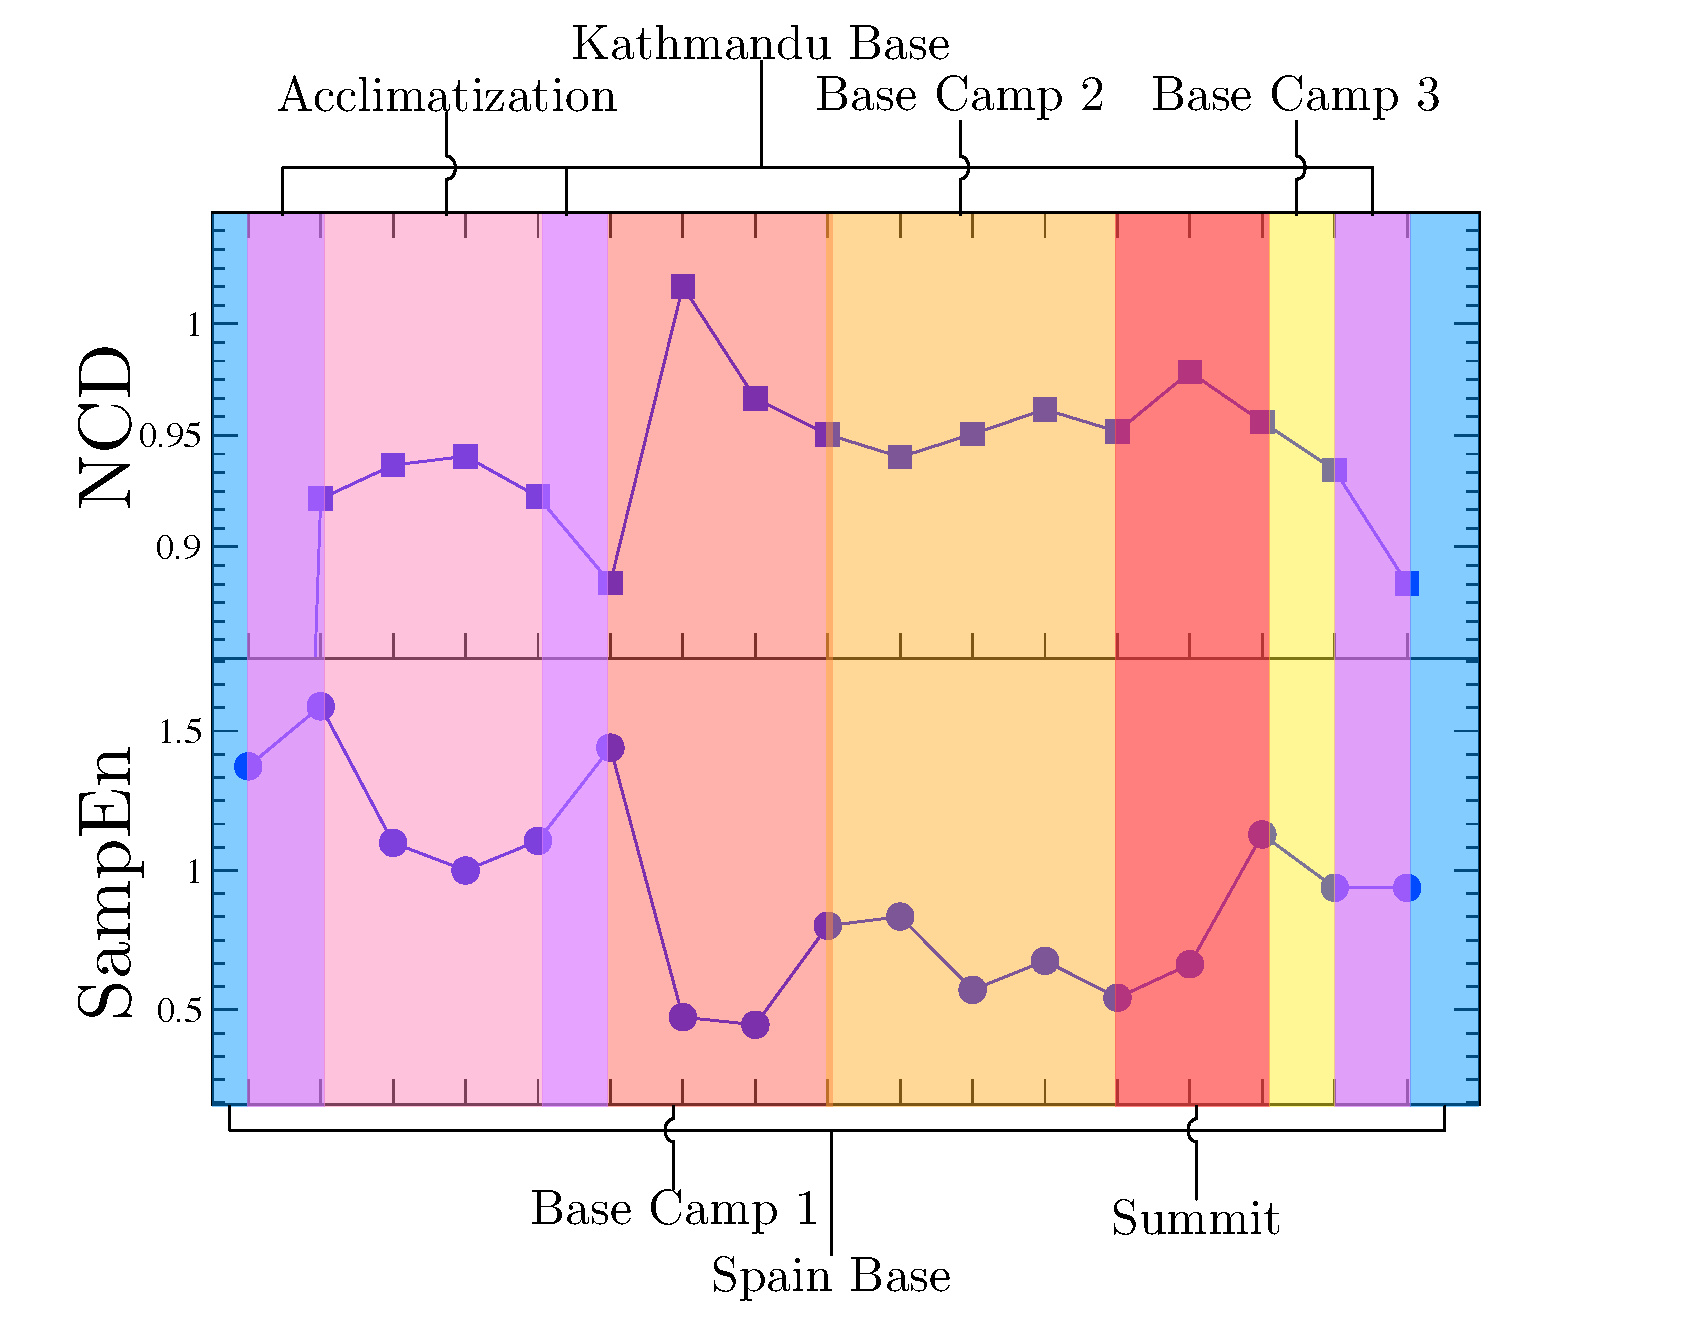
\includegraphics[width=0.9\textwidth]{./figs/Fig1_ST}\\[-0.1cm]
  \end{center}
  \caption{\emph{\small NCD and SampEn evolution during the expedition for one climber.}}
\end{figure*}




